\documentclass{beamer}
\usepackage[utf8]{inputenc}
\usepackage[T1]{fontenc}
\usepackage{mathpazo}
\usepackage{eulervm}
\usepackage{natbib}
\usepackage{amsfonts}
\usepackage{amsmath}



\usepackage{tikz}
\usepackage{verbatim}
\usetikzlibrary{arrows,shapes,decorations.pathmorphing}



% New commands to keep things tidy.
\newcommand{\vp}[0]{\vec{p}}
\newcommand{\vk}[0]{\vec{k}}
\newcommand{\ket}[1]{|#1\rangle}
\newcommand{\bra}[1]{\langle#1|}
\newcommand{\Om}[1]{\small $\omega_{#1}$}
\newcommand{\De}[1]{$\Delta_{#1}$}
\newcommand{\Ga}[1]{$\Gamma_{#1}$}
\newcommand{\pauli}[1]{\sigma_{#1}}

\usetheme{Dresden}
\usefonttheme{serif}
\usecolortheme{rose}



\title{Struggles in Science:}
\author{Maeve Andersen}

\begin{document}
\setcitestyle{authoryear,round,comma,aysep={;},yysep={,},notesep={, }}
% For every picture that defines or uses external nodes, you'll have to
% apply the 'remember picture' style. To avoid some typing, we'll apply
% the style to all pictures.
\tikzstyle{every picture}+=[remember picture]

% By default all math in TikZ nodes are set in inline mode. Change this to
% displaystyle so that we don't get small fractions.
\everymath{\displaystyle}

\maketitle

\frame{\tableofcontents}

\section{Science!}
\subsection{How do we think of light matter coupling?}
\subsection{Treatments of Light Matter}
\begin{frame}{Scully's Explanation (Semi-Classical)}
     \citep{Scully1997} describes this in chapter 5.C:Quasimode laser physics based on the modes of the universe
    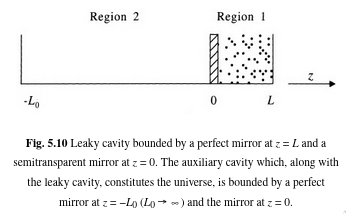
\includegraphics{scully/scully_universe_mirrors.png}
\end{frame}



\section{Science?}
\begin{frame}{My entire social life changed, and that was hard}

When I came out, my social identity changed non-adiabatically. I had to build a new social life as a new person. It was one of the hardest things I've ever done.
\end{frame}


\begin{frame}{I accumulated a lot of trauma from wearing dresses and makeup everyday}
At age 24, I felt really really **really* awkward trying to be myself public. I knew that it was okay for me to wear dresses to work, but I felt really unprofessional while doing it. I felt *incompetent* in how I expressed myself.
\end{frame}

\begin{frame}{Face dysphoria sucked and still does!}
I have face dysphoria and I was *really* bad when I first transitioned. I got a pretty shocked response when i showed up to the office in this. 
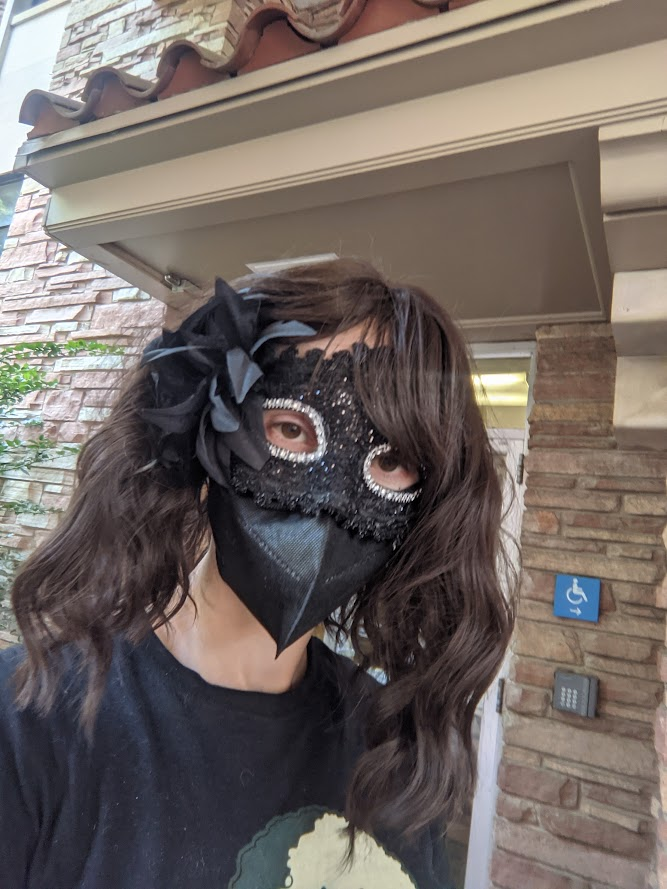
\includegraphics{mae_pics/mae_mask.jpg}

\includegraphics{mae_pics/mae_umbrella.jpg}  
\end{frame}


\end{document}
